\section{Pruebas}
\subsection{Prueba de propiedad \ref{p1}}
\label{subsection:proof1}
\begin{proof}
	Sin pérdida de la generalidad, podemos asumir que las \textit{ponderaciones} con los que el votante $a_i$
	valúa todas las {\dapp}s son $b_{i1}, b_{i2}, \ldots, b_{in}$ respectivamente, y que son valores fijos. Asumimos que los valores de contribución del votante $a_i$ a todas las {\dapp}s son
	$\nr_{i1},\ldots,\nr_{in}$ respectivamente, y que son ajustables por el votante $a_i$.

	El objetivo de la optimización del votante $i$ es la suma ponderada de los puntajes de las valuaciones que ofrece, definida por:
	$$w_i = \sum_{j=1}^n b_{ij}\sqrt{\nr_{ij}}$$
	De acuerdo a la inecualidad de Cauchy, se desprende que:
	$$w_i = \sum_{j=1}^n b_{ij}\sqrt{\nr_{ij}} \leq (\sum_{j=1}^n b_{ij}^2)(\sum_{j=1}^n \nr_{ij}) \leq (\sum_{j=1}^n b_{ij}^2)\nr_i$$
	El último término del segundo miembro en la ecuación de arriba es un valor fijo. La igualdad se mantiene sí y sólo sí:
	$$\frac{b_{i1}^2}{\nr_{i1}}=\frac{b_{i2}^2}{\nr_{i2}}=\cdots=\frac{b_{in}^2}{\nr_{in}}$$
	Así, la propiedad queda demostrada.
\end{proof}

\subsection{Prueba de propiedad \ref{p2}}
\label{subsection:proof2}
\begin{proof}
	Sin pérdida de la generalidad, se asume que el desarrollador de la dapp $d_1$ la divide en dos {\dapp}s. Para todo votante normal que pertenece al segundo caso descripto en la sección \ref{subsec:5.2} asumiendo que las \textit{ponderaciones} asignados a valuar las
	{\dapp}s antes de su división son $b_{i1},b_{i2},\ldots,b_{in}$ y las ponderaciones con los que valúa las dos {\dapp}s divididas son $b'_{i1},b'_{i2}$, se sostiene que $b_{i1} \geq b'_{i1}+b'_{i2}$ de acuerdo a nuestra presunción.

	Luego, computamos los valores de contribución del votante $a_i$ antes de ocurrir la división. Se define $H_i = \sum_{j=2}^n b_{ij}^2$, de acuerdo a la conclusión en la propiedad \ref{p1} y de acuerdo al Teorema de Particiones tenemos:
		 $$\frac{\nr_{i1}}{b_{i1}^2} = \frac{\sum_{j=1}^n \nr_{ij}}{\sum_{j=1}^n b_{ij}^2} = \frac{\nr_i}{b_{i1}^2+H_i}$$
  Similarmente, el valor de contribuciones del votante $a_i$ a la $t$-a división de la \dapp (denotada por $\nr'_{it},t=1,2$) es:
  	 $$\nr'_{it} =  \frac{b_{it}^{'2}\nr_i}{b_{i1}^{'2}+b_{i2}^{'2}+H_i}$$
  	 Nótese que $b_{i1}^2 \geq (b‘_{i1}+b’_{i2})^2 >b_{i1}^{'2}+b_{i2}^{'2}$, tenemos
  	 $$\nr_{i1} > \nr'_{i1}+\nr'_{i2}$$
  	 Así, introducimos la restricción de los valores de contribución para un votante lo suficientemente racional. Generalmente, la mayoría de los votantes pertenece al primer caso descripto en la sección \ref{subsec:5.2}, esto es, sencillamente distribuyen los valores de contribución que se suponen para $d_1$ para las {\dapp}s divididad. En cualquier caso, tenemos:
  	 	 	$$\nr_{i1} \geq \nr'_{i1}+\nr'_{i2}$$
  	 Defínase $S'_1,S'_2$ como los dos puntajes de valuación de las {\dapp}s, respectivamente. Por definición:
  	 	 $$S'_1 =  \sum_{i=1}^m \sqrt{\nr'_{i1}},~~~S'_2 =  \sum_{i=1}^m \sqrt{\nr'_{i2}},~~~S_1 = \sum_{i=1}^m \sqrt{\nr_{i1}}$$
  	Defínase $U'_1$ como el incentivo final del desarrollador de la \dapp $d_1$ luego de la división. Por definición:
  		 $$U'_1=\frac{S_1^{'2}+S_2^{'2}}{S_1^{'2}+S_2^{'2}+\sum_{j=2}^n S_j^2} \lambda M,~~~U_1=\frac{S^2_1}{S_1^2+\sum_{j=2}^n S_j^2} \lambda M$$
  	Nótese que dados $S_2,\ldots,S_n$,
  		 $$ U_1 \geq U'_1 \Leftrightarrow S_1^2 \geq S_1^{'2}+S_2^{'2}$$
   Para mostrar si la división aumenta la utilidad, sólo es necesario comparar los siguientes dos términos:
   	 $$S_1^2 = (\sum_{i=1}^m \sqrt{\nr_{i1}})^2,~~~S_1^{'2}+S_2^{'2}=  (\sum_{i=1}^m \sqrt{\nr'_{i1}})^2+(\sum_{i=1}^m \sqrt{\nr'_{i2}})^2$$
   	En realidad, $S_1^2 \geq S_1^{'2}+S_2^{'2}$ pueden ser demostrados de acuerdo al teorema de la distancia más corta.
   		 \begin{figure}
   		 	\centering
   		 	%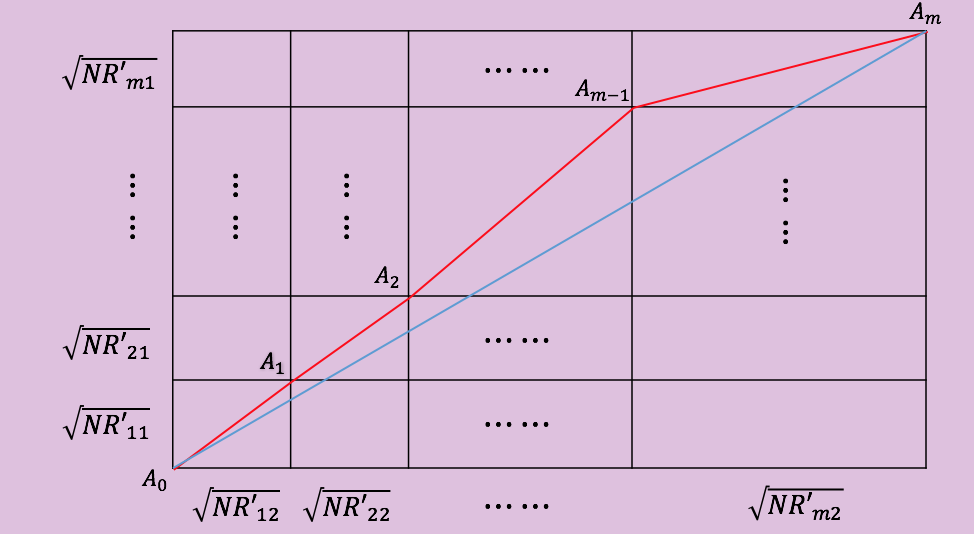
\includegraphics[width = 0.6\textwidth]{../common/m1.png}
   		 	\begin{tikzpicture}
\pgfmathsetmacro{\HEIGHT}{1.2}
\pgfmathsetmacro{\HDOT}{2.2}
\pgfmathsetmacro{\WDOT}{3.2}
\pgfmathsetmacro{\WOne}{1.6}
\pgfmathsetmacro{\WTwo}{2.2}
\pgfmathsetmacro{\WN}{4.2}

\pgfmathsetmacro{\LEN}{\WOne + \WTwo + \WN + \WDOT}
\pgfmathsetmacro{\TH}{3*\HEIGHT+ \HDOT}

\tikzset{
  t/.style={draw, on grid, align=center, minimum height=1ex},
  coord/.style={coordinate, on grid, node distance=6mm and 25mm},
  between/.style args={#1 and #2}{
         at = ($(#1)!0.5!(#2)$)
    }
}

\draw [name path=h1] (0, 0) -- (\LEN, 0);
\draw [name path=h2] (0, \HEIGHT) -- (\LEN, \HEIGHT);
\draw [name path=h3] (0, 2*\HEIGHT) -- (\LEN, 2*\HEIGHT);
\draw [name path=h4] (0, 2*\HEIGHT + \HDOT) -- (\LEN, 2*\HEIGHT + \HDOT);
\draw [name path=h5] (0, 3*\HEIGHT + \HDOT) -- (\LEN, 3*\HEIGHT + \HDOT);

\draw[name path=v1] (0, 0) -- (0, \TH);
\draw[name path=v2] (\WOne, 0) -- (\WOne, \TH);
\draw[name path=v3] (\WOne + \WTwo, 0) -- (\WOne + \WTwo, \TH);
\draw[name path=v4] (\WOne + \WTwo + \WDOT, 0) -- (\WOne + \WTwo + \WDOT, \TH);
\draw[name path=v5] (\WOne + \WTwo + \WDOT + \WN, 0) -- (\WOne + \WTwo + \WDOT + \WN, \TH);

\path [name intersections={of=h1 and v1,by=A0}];
\path [name intersections={of=h2 and v2,by=A1}];
\path [name intersections={of=h3 and v3,by=A2}];
\path [name intersections={of=h4 and v4,by=Am1}];
\path [name intersections={of=h5 and v5,by=Am}];

\draw [red] (A0) -- (A1) -- (A2) -- (Am1) -- (Am);
\draw [blue] (A0) -- (Am);

\node [below=0.01 of A0, anchor=north east] {$A_0$};
\node [above=0.05 of A1, anchor=south east]{$A_1$};
\node [above=0.05 of A2, anchor=south east] {$A_2$};
\node [above=0.05 of Am1, anchor=south east] {$A_{m-1}$};
\node [above=0.05 of Am, anchor=south]{$A_m$};


\path [name intersections={of=h1 and v1,by=t00}];
\path [name intersections={of=h2 and v1,by=t01}];
\path [name intersections={of=h3 and v1,by=t02}];
\path [name intersections={of=h4 and v1,by=t03}];
\path [name intersections={of=h5 and v1,by=t04}];
\node [coord, between=t00 and t01] (x1){};
\node [coord, between=t01 and t02] (x2){};
\node [coord, between=t02 and t03] (x3){};
\node [coord, between=t03 and t04] (x4){};

\node [left=0.05 of x1.west] {$\sqrt{{\nr}'_{11}}$};
\node [left=0.05 of x2.west] {$\sqrt{{\nr}'_{21}}$};
\node [left=0.7 of x3.west, anchor=center] {$\vdots$};
\node [left=0.05 of x4.west] {$\sqrt{{\nr}'_{m1}}$};

\path [name intersections={of=h1 and v1,by=s00}];
\path [name intersections={of=h1 and v2,by=s01}];
\path [name intersections={of=h1 and v3,by=s02}];
\path [name intersections={of=h1 and v4,by=s03}];
\path [name intersections={of=h1 and v5,by=s04}];
\node [coord, between=s00 and s01] (y1){};
\node [coord, between=s01 and s02] (y2){};
\node [coord, between=s02 and s03] (y3){};
\node [coord, between=s03 and s04] (y4){};

\node [below=0.5 of y1.south, anchor=center] {$\sqrt{{\nr}'_{12}}$};
\node [below=0.5 of y2.south, anchor=center] {$\sqrt{{\nr}'_{22}}$};
\node [below=0.5 of y3.south, anchor=center] {$\dots$};
\node [below=0.5 of y4.south, anchor=center] {$\sqrt{{\nr}'_{m2}}$};

\node at (x1.east -| y3.north) {$\dots$};
\node at (x2.east -| y3.north) {$\dots$};
\node at (x4.east -| y3.north) {$\dots$};

\node at (y1.north |- x3.east) {$\vdots$};
\node at (y2.north |- x3.east) {$\vdots$};
\node at (y4.north |- x3.east) {$\vdots$};

\end{tikzpicture}

   		 	\caption{Prueba de la distancia más corta\label{fig:path}}
   		 \end{figure}
   Como se muestra en la figura \ref{fig:path}, construimos una grilla cuyos largo y ancho están divididos en $m$ segmentos, cuyo $i$-ésimo segmento tiene una longitud de $\sqrt{\nr'_{i1}}$ y $\sqrt{\nr'_{i2}}$ respectivamente.

   	Entonces, $S_1^{'2}+S_2^{'2}=A_0A_m^2$, esto es, es igual al cuadrado de la longitud del segmento azul. Entretanto,
   	 $$S_1^2 = (\sum_{i=1}^m \sqrt{\nr_{i1}})^2 > (\sum_{i=1}^m \sqrt{\nr'_{i1}+\nr'_{i2}})^2 = (\sum_{i=1}^m A_{i-1}A_i)^2$$,
   	 que es igual a la suma de los cuadrados de todos los segmentos rojos. Como la distancia más corta entre dos puntos es un segmento lineal, se mantiene que $S_1^2 >S_1^{'2}+S_2^{'2}$.

   	 Para los casos en los que las {\dapp}s $k>2$ están divididas, podemos considerarlo como divisiones sucesivas y usar iterativamente el resultado en $k=2$.

   	 Así, la propiedad queda probada.

\end{proof}

\subsection{Prueba de corolario \ref{c1}}
\label{subsection:proof3}
\begin{proof}
	Para todo votante comprado por el desarrollador de una \dapp $d_1$, antes de su división, podemos considerar al votante como un votante normal que valúa todas las {\dapp}s con un vector de ponderación $(1,0,0,\ldots,0)$, ya que otorga toda su capacidad de voto a $d_1$.
	Suponemos ahora que $d_1$ se divide en $k$ {\dapp}s y que los valores de contribución de los votantes comprados a las {\dapp}s $k$ son $\nr_{t1},\ldots,\nr_{tk}$, cuya suma es fija. De acuerdo a la condición de que la igualdad se mantenga para la inecualidad de Cauchy en la Prueba de Propiedad \ref{p1}, el votante puede ser considerado como un votante normal que valúa todas las {\dapp}s con un vector de ponderación
	$(\sqrt{\nr_{t1}}/C,\sqrt{\nr_{t2}}/C,\ldots, \sqrt{\nr_{tk}}/C,0,0,\ldots,0)$, donde $C=\sum_{j=1}^k \sqrt{\nr_{tj}}$. Esto es, el votante valúa las {\dapp}s divididas con ponderaciones de acuerdo a proporción, y valúa todas las otras {\dapp}s con ponderaciones 0.\footnote{Nótese que al escalar todas las ponderaciones mediante una constante no se afectan los resultados, ya que el valor de contribución total del votante sólo depende de las proporciones de las ponderaciones con respecto a las ponderaciones totales}. Como
		$$\sum_{j=1}^k \sqrt{\nr_{tj}}/C =1$$
	por lo que el caso de este corolario puede reducirse al caso de los votantes normales. (Propiedad\ref{p2}). Así, el corolario queda probado.
\end{proof}

\subsection{Prueba de propiedad \ref{p3}}
\begin{proof}
	Consideramos en primer lugar el caso de un votante que divide su cuenta en dos sub-cuentas. Consideramos $c$ como la cuenta original y $a,b$ como las sub-cuentas, $S,S'$ son las puntuaciones de valoración de la \dapp que el votante planea votar antes y después de la división respectivamente, $U,U'$ son los incentivos finales para el desarrollador de la \dapp que el votante planea votar, antes y después de la división respectivamente. Por definición, tenemos
	$$S= \sqrt{\nr_c}+O,\quad S'=\sqrt{\nr_a}+\sqrt{\nr_b}+O$$,
	donde $O$ es la suma de los valores de contribución de otros votantes, que es un valor fijo.

	Mediante ~\ref{eq:sqrt_nr} se sostiene que $S < S'$. Esto es, la valuación de la \dapp no se incrementa.

	Entretanto, por definición,
	$$U = \frac{S}{S+P}\lambda M,\quad U' = \frac{S'}{S'+P} \lambda M$$,
	donde $P$ es la suma de los cuadrados de los puntajes de la valuación de las otras \dapp, cuyo valor es fijo.

	Como $S < S'$ se sostiene que $U \leq U'$. Esto es, el incentivo final que recibe el desarrollador no se incrementa.

	Para los casos en los que $k>2$ cuentas están divididas, podemos considerarlo como divisiones sucesivas y usar iterativamente el resultado en $k=2$.

\end{proof}